\documentclass[a4paper]{article}
%\usepackage[subpreambles=true]{standalone}
\usepackage[utf8]{inputenc}
\usepackage[T1]{fontenc}
\usepackage[spanish]{babel}

% \usepackage{tikz}
\usepackage{tikz,tikz-3dplot} 
\usepackage{tkz-euclide}
% \usetkzobj{all}

\usepackage{upgreek}  % \varsigma \upvarsigma ... etc
\usepackage{tipa}  % \textbullseye
\usepackage{multicol}
\usepackage{graphicx}
\usepackage{subcaption}
\usepackage{booktabs}
\usepackage{amsmath}
\usepackage{listings}
\usepackage{xcolor}
\usepackage{float}  % \begin{figure}[H]

\usepackage{geometry}

%\lstset { %
%%    language=C++,
%    backgroundcolor=\color{black!10}, % set backgroundcolor
%%    breaklines=true,
%%    frame=tlbr,
%    xleftmargin=0.5cm,
%    basicstyle=\ttfamily,
%    basicstyle=\footnotesize,% basic font setting
%}

\lstdefinestyle{customc}{
  belowcaptionskip=1\baselineskip,
  breaklines=true,
  frame=L,
  xleftmargin=\parindent,
  language=C++,
  morekeywords={*, Int_t, UInt_t, Float_t, Bool_t, TMatrixF, TString, ClonesArray, TClonesArray}, 
  numbers=left,
  showstringspaces=false,
  basicstyle=\footnotesize\ttfamily,
  keywordstyle=\bfseries\color{green!40!black},
  commentstyle=\itshape\color{purple!40!black},
  backgroundcolor=\color{yellow!10},
  identifierstyle=\color{black},
  stringstyle=\color{orange}\itfamily,
}

\lstdefinestyle{customsh}{
  language=bash,
  basicstyle=\color{green!60}\small\ttfamily,
  numbers=left,
  numberstyle=\color{black}\small\ttfamily,
  numbersep=3pt,
  frame=tb,
  showstringspaces=false,
  breaklines=true,
  columns=fullflexible,
  backgroundcolor=\color{black!85},
  linewidth=0.9\linewidth,
  xleftmargin=\parindent,  % 0.05\linewidth,
  xrightmargin=-0.1\linewidth
}

\usepackage{hyperref}
\usepackage{breakurl}

\let\vec\mathbf  % Bold vectors

\graphicspath{{images/}}

\usepackage[edges]{forest}
\definecolor{folderbg}{RGB}{124,166,198}
\definecolor{folderborder}{RGB}{110,144,169}
\newlength\Size
\setlength\Size{4pt}
\tikzset{%
  folder/.pic={%
    \filldraw [draw=folderborder, top color=folderbg!50, bottom color=folderbg] (-1.05*\Size,0.2\Size+5pt) rectangle ++(.75*\Size,-0.2\Size-5pt);
    \filldraw [draw=folderborder, top color=folderbg!50, bottom color=folderbg] (-1.15*\Size,-\Size) rectangle (1.15*\Size,\Size);
  },
  file/.pic={%
    \filldraw [draw=folderborder, top color=folderbg!5, bottom color=folderbg!10] (-\Size,.4*\Size+5pt) coordinate (a) |- (\Size,-1.2*\Size) coordinate (b) -- ++(0,1.6*\Size) coordinate (c) -- ++(-5pt,5pt) coordinate (d) -- cycle (d) |- (c) ;
  },
}
\forestset{%
  declare autowrapped toks={pic me}{},
  declare boolean register={pic root},
  pic root=0,
  pic dir tree/.style={%
    for tree={%
      folder,
      font=\ttfamily,
      grow'=0,
    },
    before typesetting nodes={%
      for tree={%
        edge label+/.option={pic me},
      },
      if pic root={
        tikz+={
          \pic at ([xshift=\Size].west) {folder};
        },
        align={l}
      }{},
    },
  },
  pic me set/.code n args=2{%
    \forestset{%
      #1/.style={%
        inner xsep=2\Size,
        pic me={pic {#2}},
      }
    }
  },
  pic me set={directory}{folder},
  pic me set={file}{file},
}


\begin{document}

\begin{centering}

\begin{minipage}[c]{0.4\linewidth}
    \centering

\includegraphics[height=5\baselineskip]{LogoUSC}
\end{minipage}

	\vspace{1.5cm}
    {\huge\bfseries Reconstrucci\'on de trazas en detectores tipo \textsc{Trasgo} para la medida de rayos cósmicos:\\
    Detectores TRAGALDABAS y STRATOS
    \par}
  
\vspace{0.5cm}

{\Large  Sara Costa, Miguel Cruces,   Juan A. Garzón}
	
	\vspace{0.5cm}

	{\large\bfseries LabCAF / IGFAE  \par Universidade de Santiago de Compostela}

	\vspace{1cm}

\end{centering}


% \tableofcontents


% \textsc{todo}: 
% \begin{itemize}
%     \item Rasayos cósmicos:
%     \begin{itemize}
%         \item (Yanis 17) Flujo de partículas compuesto en mayor parte por protones y núcleos atómicos con rangos de energía $(10^8, 10^{20})$ eV (o mayores).
%         \item Yanis figura 1.7 (buscar referencia real). Flujo vertical de secundarios: llegan muchos muones (neutrinos indetectables), protones (neutrones indetectables) y algunos electrones (la mayoría se generan en el edificio supongo).
%         \item Describir lo que es una saeta: Conjunto de parámetros $\vec{r}_k = (x_k, x_k', y_k, y_k', t_k, 1/v)^T$
%     \end{itemize}
%     \item TRAGALDABAS:
%         \begin{itemize}
%             \item Localización y dimensiones (pg 54)
%             \item Ratio de 80 Hz? (pg 55)
%         \end{itemize}
%     \item Simulación:
%         \begin{itemize}
%             \item Distribuciñon angular, temporal, lentitudes, 
%         \end{itemize}
% \end{itemize}

\section{Introducción}

Presentamos en este informe un resumen de las actividades realizadas para la puesta a punto de un programa para la reconstrucción de trazas en detectores tipo \textsc{trasgo}, en particular para los detectores del proyecto \textsc{stratos}. Para ello se ha adaptado y mejorado una cadena de programas existente, GENEDITIGTANA, que genera datos aleatorios, los digitaliza y, finalmente, los reconstruye, permitiendo estimar tanto la aceptancia mo la resolución de la reconstrucción realistas asociadas a un detector. Como novedad, hemos introducido la posibilidad de buscar candidatos a trazas mediante un algoritmo de filtrado de Kalman. Esto permitirá separar y reconstruir las cascada electromagnéticas asociadas a electrones y gammas, tarea imprescindible para los estudios atmosféricos que pretendemos, con una gran eficacia.

\section{Los detectores tipo  \textsc{trasgo} y la atmósfera}

El desarrollo de la tecnología RPC (Resistive Plate Chambers) propia de experimentos de Física Nuclear  y de Física de Partículas de Altas Energías y ha abierto la posibilidad de diseñar y construir detectores de rayos cósmicos de nueva generación capaces de medir con gran precisión haces de electrones de alta multiplicidad y muones de origen cósmico a nivel del suelo. Sin duda, la propuesta mas interesante de dicho tipo de detectores a nivel mundial la constituyen los detectores tipo \textsc{trasgo} \cite{jag, moscu}, desarrollados por la Universidad de Santiago de Compostela en colaboración con el LIP de Coimbra.  Las empresas HIdronav  y Digafer han tenido una papel muy  destacado, proporcionando soporte técnico, material electrónico y desarrollo instrumental. Fruto de ello han sido los detectores \textsc{tragaldabas}, actualmente tomando datos en la Univ. de Santiago de Compostela, el detector \textsc{tristan}, instalado en una base española en la Antártida, y el detector \textsc{mutt}, que estuvo instalado en los locales de Digafer, cerca de Porriño, siendo pionero en usar la tecnología de RPCs para la realización de tomografía mediante rayos cósmicos. Finalmente, el proyecto \textsc{Stratos} constituye un salto adelante muy importante pues reúne gran parte de la experiencia adquirida en los proyecto anteriores con el desarrollo de una nueva familia de detectores con prestaciones en posición, reconstrucción angular y resolución angular muy por encima de los conseguidos en los detectores previos.

Es bien conocido el importante efecto que las condiciones atmosféricas, en particular la presión y el perfil de temperaturas de la atmósfera sobre el detector, ejercen sobre el resultado de la  medida de rayos cósmicos medidos en tierra. En particular, es muy interesante la correlación observada entre la tasa de muones de muy alta energía medida en tierra y la temperatura efectiva de la atmósfera, en la que dominan las variaciones de la temperatura en la estratosfera. Ello abre la posibilidad de aprovechar las magníficas prestaciones que ofrecen los detectores tipo \textsc{trasgo}, capaces de acceder a información vedada a los detectores de rayos cósmicos tradicionales, para estimar en tiempo real el perfil de temperaturas de la atmósfera en la vertical del detector. 
Esta posibilidad conlleva la necesidad de desarrollar y poner a punto algoritmos novedosos de reconstrucción de la dirección de llega de electrones y muones y que, además, permitan tanto su identificación como incluso la estimación de la energía de las cascadas electromagnéticas inducidas por los electrones de alta energía.


% \begin{figure}
%   \centering
%   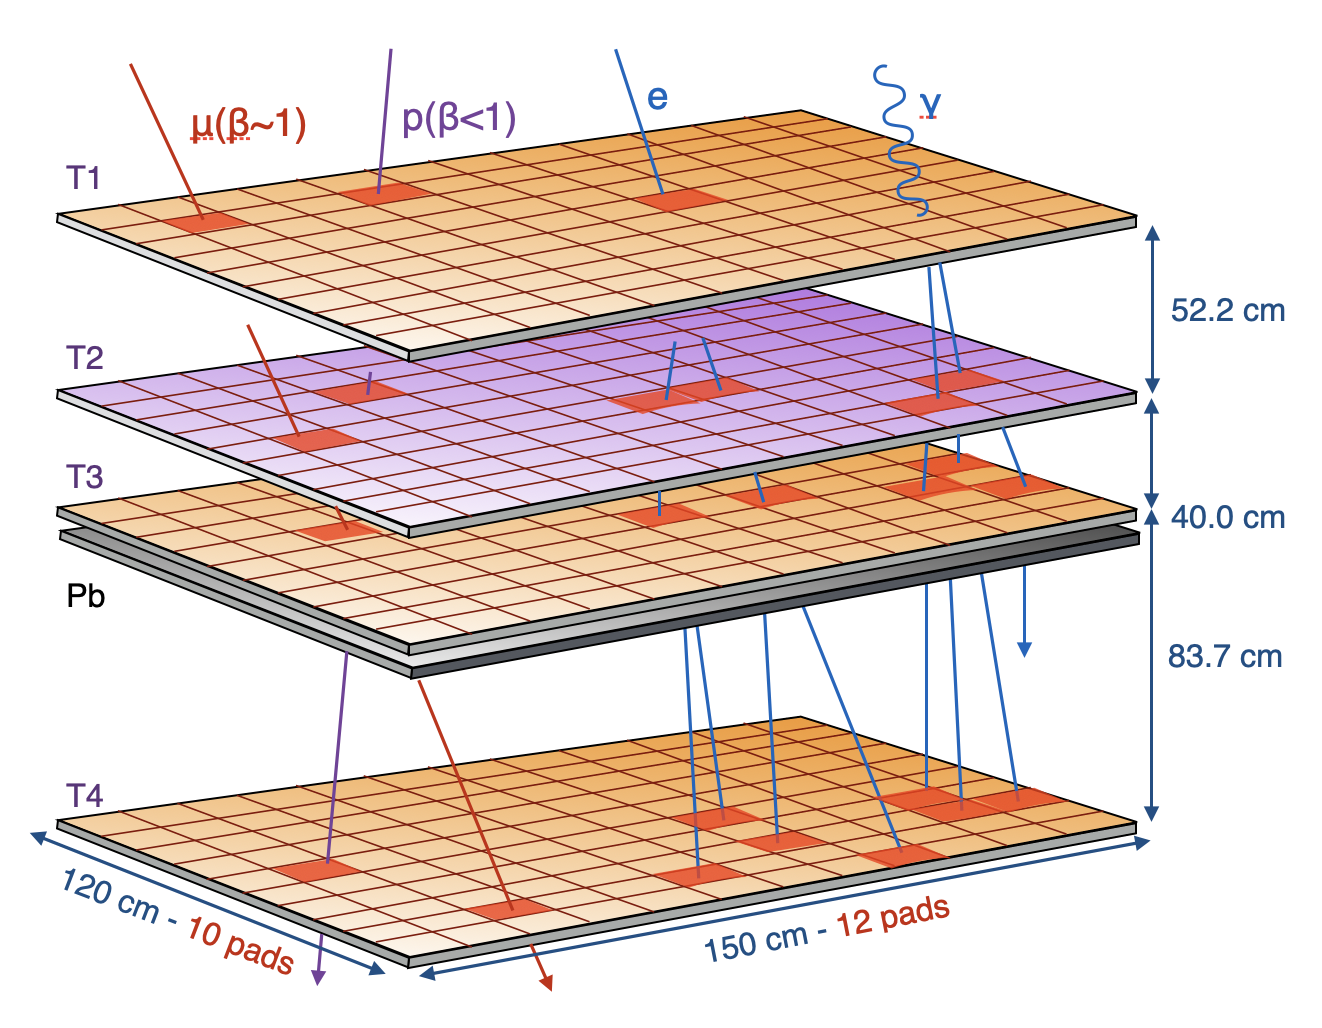
\includegraphics[width=\linewidth]{tragas_3d.png} 
%   \caption{Representación del detector \textsc{tragaldabas} en su versión con cuatro RPCs. Partículas con distinta naturaleza dejan una huella diferente en el detector.}
%   \label{fg:trag3d} 
% \end{figure}


\begin{figure}[h] 
  \centering
  \begin{subfigure}[c]{0.45\linewidth}
    \centering
    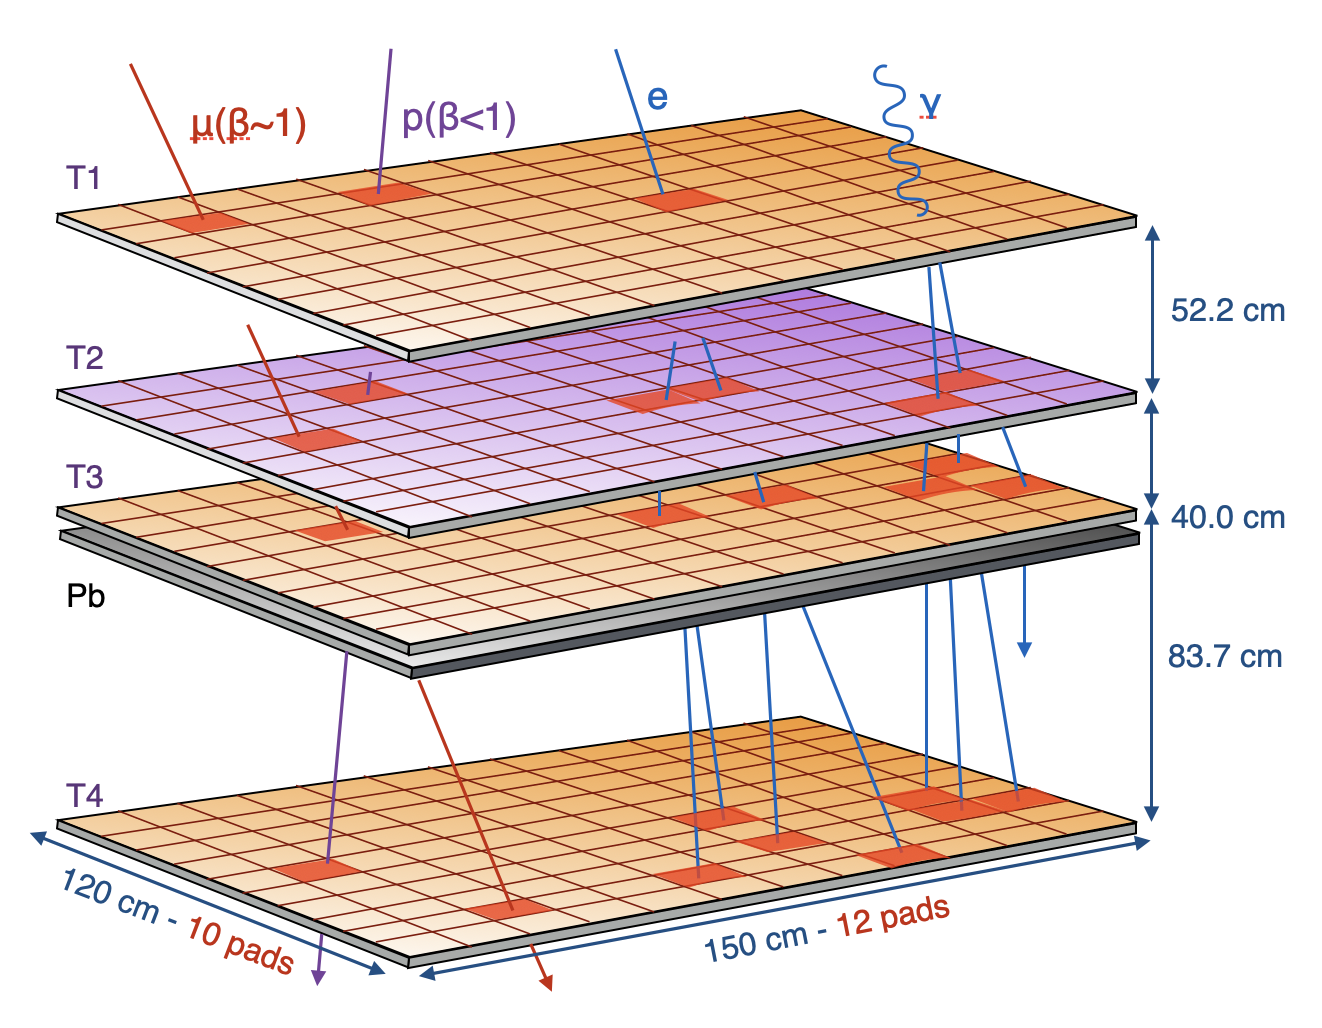
\includegraphics[width=\linewidth]{tragas_3d.png} 
    \caption{Diferentes tipos de partículas muestran diferentes topologías típicas a su paso por el detector.}
    \label{fg:intro1-a} 
  \end{subfigure} 
  \hspace{0.2cm}
  \begin{subfigure}[c]{0.50\linewidth}
    \centering
    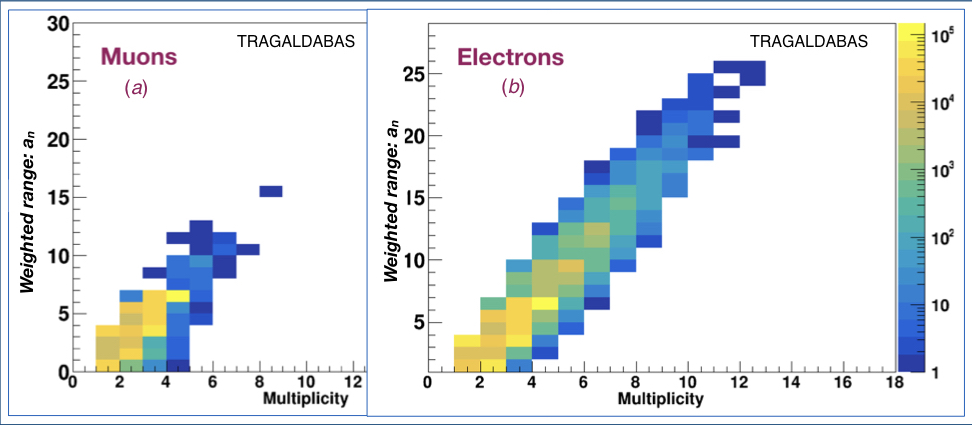
\includegraphics[width=\linewidth]{b_midasp.jpeg} 
    \caption{Ejemplo de cómo la medida del número de celdas impactadas y el alcance ponderado de las trazas permiten separar electrones de muones.} 
    \label{fg:intro1-b} 
  \end{subfigure}%% 
  \caption{Ejemplo de la capacidad de identificación de los detectores de tipo \textsc{trasgo}, aplicada al detector  \textsc{tragaldabas} de la USC.}
  \label{fg:intro1} 
\end{figure}

La figura \ref{fg:intro1-a} resume el fundamento de la capacidad de los detectores tipo \textsc{trasgo} para la identificación de los diferentes tipos de partículas. En relación con la separación entre muones y electrones, es de destacar que mientras los primeros deben de producir trazas rectilíneas proporcionando un buen ajuste, los electrones de alta energía tienen tendencia a producir cascadas electromagnéticas formadas por nuevos electrones y gammas activando un número elevado de electrodos. Dicho efecto queda bien reflejado en los resultados de simulación que se muestran en la figura \ref{fg:intro1-b}. En ella se observa la capacidad que un detector tipo \textsc{trasgo} ofrece para separar electrones y muones analizando algunos observables; en concreto, el valor del chi cuadrado del ajuste, el numero de celdas activadas y el alcance ponderado, que tiene en cuenta la distribución longitudinal de las celdas activadas. La capacidad de distinguir electrones de muones alcanza valores que superan el 90 por ciento.

TimTrack \cite{ttrack} y el filtrado de Kalman \cite{joaneh} son dos herramientas de reconstrucción de trazas ideales para sacar provecho de la magníficas prestaciones que ofrecen los detectores tipo \textsc{trasgo}. La primera de ellas fue desarrollada específicamente para este tipo de detectores mientras que la segunda constituye un estándar ampliamente utilizado en la ciencia y en la técnica. Hemos aplicado ambas herramientas al desarrollo de un programa de reconstrucción de haces de partículas, necesario para su uso en el proyecto \textsc{stratos}, si bien lo hemos aplicado también a la estructura en electrodos planos del detector \textsc{tragaldabas} de la Univ. de Santiago de Compostela, ya que para él disponemos de datos reales. Para ello nos hemos ayudado de la cadena de programas \textit{genedigitana}, que permite simular la respuesta de un detector cualquiera a la incidencia de partículas cargadas y proceder después a su reconstrucción y estimar la incertidumbre de los parámetros de la partícula incidentes, junto con su matriz de correlación.

%El detector está basado en la tecnología \textsc{rpc}\footnote{Resistive Plate Chamber} que ofrece una superficie de 1.8 m$^2$ con granularidad de 120 celdas, capacidad de multitracking, resolución temporal entorno a 0.4 ns, con una resolución angular cerca de los 3$^\circ$ y aceptancia angular de 40$^\circ$.


\section{Genedigitana}

\textit{GENEDIGITANA} es el acrónimo de las tres palabras generación, digitalización y análisis y llamamos así a un programa,  o cadena de subprogramas, desarrollado en el LabCAF y disponible en \textsf{Mathematica} y en \textsf{Python} y que puede ser usado para el estudio de las prestaciones de cualquier detector de partículas de configuración conocida. El programa permite incluir efectos como zonas muertas en los detectores, ineficiencias o ruido de cualquier tipo, siendo así extremadamente útil para la simulación realista de un cierto detector. 

Hemos partido de un script previo en \textsf{Python} de \textit{GENEDIGITANA}, acomodándolo para aplicar el proceso a la estructura de los detectores \textsc{tragaldabas} y  \textsc{stratos}. También hemos ampliado el código para añadir nuevas funcionalidades y mayor flexibilidad y robustez.

La cadena \textit{genedigitana} consta de tres procesos:

\begin{itemize}
    \item Generación: construcción aleatoria de rectas en tres dimensiones que emulan trayectorias de partículas que se mueven a una cierta velocidad e incidiendo en el detector en un cierto instante de tiempo.
        
    \item Digitalización: conversión de la información analítica del paso de la partícula por un detector a la respuesta  esperada que de dicho detector. Este proceso es conveniente que sea lo mas realista posible reproduciendo en lo posible todas las características conocidas del detecto, incluidas las zonas muertas o la inefiiciencia en la medida.
    Por ejemplo, en el caso de un detectores de electrodos rectangujares, o pads, como el \textsc{tragaldabas} , la respuesta esperada son las coordenadas del centro de la celda, donde se supone que está conectado el electrodo de lectura, y un tiempo que es la suma del tiempo de paso de la partícula por el electrodo mas el tiempo que necesita el pulso de la señal inducida en llegar al electrodo de lectura. 
    En el casa de un detector de electrodos longitudinales, o strips, como \textsc{stratos} la respuesta esperada es son la coordenada de un extremos del strip impactado y los  dos tiempos de llegada del pulso inducido por la llegada de la partícula a ambos extremos del electrodo. A partir de dichas dos medidas se estimarán tanto el tiempo de llegada de la partícula al electrodo como su coordenada transversal en el propio electrodo. 
    
    \item Análisis: a partir de las coordenadas digitalizadas, se reconstruyen las trazas originales mediante un algoritmo, que inicialmente era TimTrack y en el que hemos incluido la posibilidad de usar un algoritmo basado en el filtrado de Kalman.
\end{itemize}

Describimos a continuación algunas de las características de la versión actual de  \textit{GENEDIGITANA} . En el apéndice se muestra una pequeña documentación de las clases utilizadas en el código informático.

\subsection{Generación}

Para definir las trazas de partículas se generan trazas, o rectas, con ángulo polar $\theta$ y ángulo acimutal $ \phi$ aleatorios, siguiendo una distribución definida por el usuario. Por defecto, lleva definida una distribución uniforme en ángulo sólido que se corresponde con una distribución uniforme en $\cos \theta$ y $\phi$, entre la vertical y un ángulo polar máximo $\theta_{max}$.
%(¿O debería ser uniforme en $\cos^2 \theta$\footnote{\url{https://www.physics.mcgill.ca/~corriveau/projects/spark/Reports/201209_blanchard_spark.pdf}}?)
El punto de incidencia $(x_0, y_0)$  se genera con distribución uniforme en cualquier punto del plano superior del detector.

Para un detector con un cierto número de planos activos para la medida de las partículas que lo atraviesan, asumimos que  existe un cierto \textit{trigger} entre planos por lo que, para simular un detector real, sólo se aceptan aquellas trazas que dejan señal en dichos planos, descartando todas las demás. Esto permite utilizar el programa también para el cálculo de aceptancias de un detector en función del tamaño del mismo y de la distancia entre los planos del trigger para una cierta distribución de partículas incidentes.

\begin{figure}[h] 
  \centering
  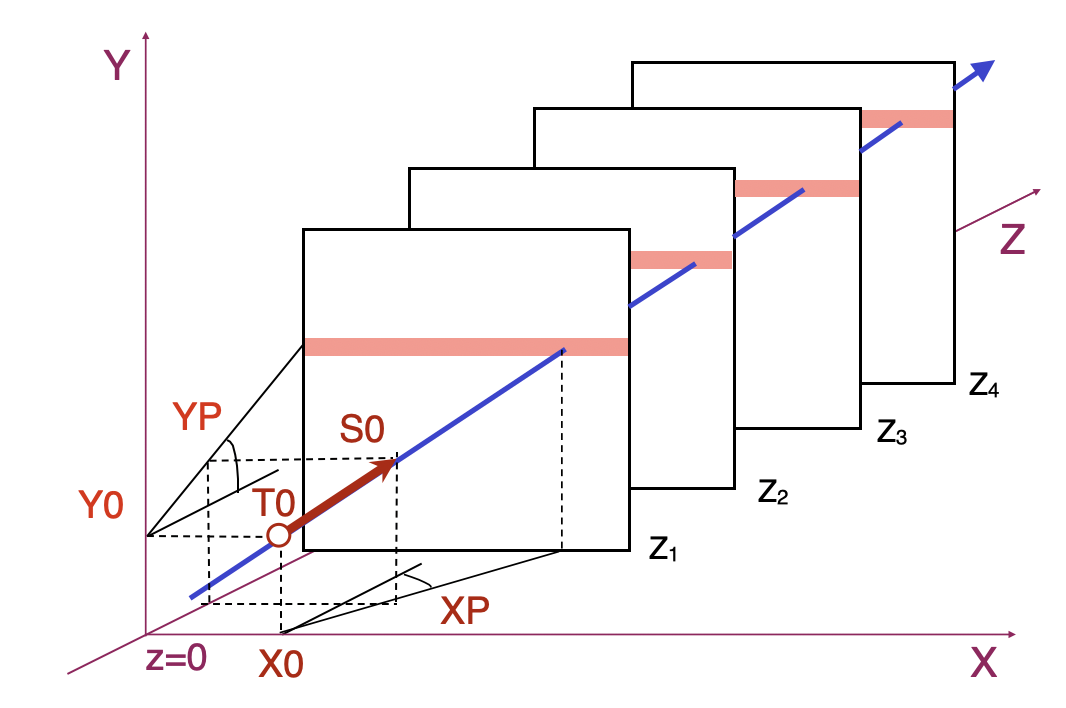
\includegraphics[width=0.7\linewidth]{saeta_3d.png} 
  \caption{Representación gráfica de una saeta.}
  \label{fg:saeta} 
\end{figure}


% \tdplotsetmaincoords{260}{340}  % Horizontal | Vertical rotations in degrees
% \begin{tikzpicture}[
%     scale=3,
%     tdplot_main_coords,
%     axis/.style={->,black,thick},
%     svector/.style={-stealth,gray,very thick},
%     vector/.style={-stealth,black,very thick},
%     vector guide/.style={dashed,gray,thick}
%     ]
%     % \tdplotsetcoord{P}{.8}{55}{60}
% 
%     % axes
%     \draw[axis]  (-0.1, 0, 0) -- (1, 0, 0)  node[anchor=south west]{$x$};
%     \draw[axis]  (0, -0.1, 0) -- (0, 1, 0)  node[anchor=south east]{$y$};
%     \draw[axis]  (0, 0, -0.1) -- (0, 0, 1)  node[anchor=north]{$z$};
% 
%     % vector
%     \pgfmathsetmacro{\ax}{0.6}
%     \pgfmathsetmacro{\ay}{0.8}
%     \pgfmathsetmacro{\az}{1.0}
%     \pgfmathsetmacro{\bx}{\ax}
%     \pgfmathsetmacro{\by}{\ay}
%     \pgfmathsetmacro{\bz}{0}
%     \draw[vector] (0,0,0) -- (\ax, \ay, \az) node[anchor=west]{$\mathrm{\textsc{Saeta}}$};
%     \draw[svector] (0,0,0) -- (\bx, \by, \bz); % node[anchor=north]{proyección};
% 
%     % dashed lines
%     \draw[vector guide] (\ax,\ay,0) -- (\ax,0,0);
%     \draw[vector guide] (\ax,\ay,0) -- (0,\ay,0);
%     \draw[vector guide] (\ax,\ay,\az) -- (\ax,\ay,0);
% 
%     % arcs
%     \tdplotdefinepoints(0,0,0)(1,0,0)(\bx,\by,\bz)
%     \tdplotdrawpolytopearc[-]{0.5}{anchor=south}{$\phi$}
% 
%     \pgfmathsetmacro{\ax}{0.6}
%     \pgfmathsetmacro{\ay}{0.8}
%     \pgfmathsetmacro{\az}{1.0}
%     \tdplotdefinepoints(0,0,0)(0,0,1)(\ax,\ay,\az)
%     \tdplotdrawpolytopearc[-]{0.75}{anchor=north}{$\theta$}
% \end{tikzpicture}

Cada traza o partícula viene caracterizada por seis parámetros que constituyen lo que llamamos una \textsc{Saeta}\footnote{SAETA:SmAllest sET of pArameters. La llamamos así porque frente a la costumbre habitual en física  de partículas de definir una partícula por su trayectoria, en nuestra aproximación, al igual que una flecha o saeta, en cada momento lleva asociada también el tiempo de paso por una cierta coordenada y su velocidad}, $\vec{s}$. 

\begin{equation}
    % \vec{s} = (\textsc{x\textbullseye}, \textsc{xp}, \textsc{y\textbullseye}, \textsc{yp}, \textsc{t\textbullseye}, \textsc{s\textbullseye})
    % \vec{s} = (\textsc{x0}, \textsc{xp}, \textsc{y0}, \textsc{yp}, \textsc{t0}, \textsc{s0})
    \vec{s} = (\textrm{X0}, \textrm{XP}, \textrm{Y0}, \textsc{YP}, \textrm{T0}, \textrm{S0})
    \label{eq:saeta}
\end{equation}

La definición de cada parámetro se muestra en la figura \ref{fg:saeta}  y es la siguiente:

\begin{itemize}
    \item X0:  Coordenada X del punto de corte de la partícula con el plano de referencia en $z=0$.
    \item XP:  Pendiente proyectada de la partícula en el plano XZ.
    \item Y0:  Coordenada Y del punto de corte de la partícula con el plano en $z=0$.
    \item YP:  Pendiente proyectada de la partícula en el plano YZ.
    \item T0:  Tiempo de paso de la partícula por el plano $z=0$, que se toma como el plano de referencia para los ajustes.
    \item S0:  Slowness o lentitud. Es la inversa del módulo de la velocidad de la partícula en el plano $z=0$,   ($\mathrm{S0} = 1/v$). Se introduce para que las ecuaciones de generación y reconstrucción de trazas guarden una cierta simetría entre la parte espacial, pares $(\mathrm{X0}, \mathrm{XP})$ y $(\mathrm{Y0}, \mathrm{YP})$, y la parte temporal, par $(\mathrm{T0}, \mathrm{S0})$. 
\end{itemize}
    
Usando la definición de los cosenos directores de una recta en el espacio que a su vez constituyen los elementos del vector unitario  en la direccion de la recta, $\vec{n} = (c_x, c_y, c_z)$, se verifica: 
\begin{align}
    \notag
    c_x & = \sin \theta \cos \phi, \\
    c_y & = \sin \theta \sin \phi, \\
    \notag
    c_z & = \cos \theta,
    % \label{eq:dir_cos}
\end{align}

y las pendientes proyectadas de una saeta se definen como:
\begin{align}
    \notag
    \mathrm{XP}& = c_x / c_z, \\
    \mathrm{YP}& = c_y / c_z.
    \label{eq:proj}
\end{align}

%Cada una de estas saetas generadas se añaden a la clase SimEvent como objetos de la clase Saeta.

\subsection{Digitalización}

Las trazas digitalizan a partir de todos aquellos puntos en los que intersectan con alguno de los planos del detector en un electrodo concreto y que como hemos visto, dependen de la geometría del detector. La información almacenada para cada intersección lo denominamos hit. Cada uno de estos hits son de clase Hit, que también se almacenan en la clase SimEvent en una lista desordenada. Esto es lo mismo que ocurre con los datos reales del detector que vienen determinados por el tiempo de llegada de las señales medidas a la electrónica de adquisición y los tiempos de retraso dentro de ésta. 

\subsection{Análisis}

El proceso de análisis consiste en reconstruir, mediante el algoritmo que se disponga y a partir de la información digitalizada proporcionada por el detector las trazas generadas y comparar la diferencia entre éstas y las generadas. Este estudio en función de los parámetros de incidencia que se desee (distribución de partículas incidentes, posición, ángulo, velocidad, etc.) permitirá estimar la resolución del detector en función de aquellos parámetros.  Así se podrán estudiar las prestaciones de un detector para distintas configuraciones y mejorar su diseño o determinar sus limitaciones.

En nuestro caso,  hemos escrito un código de reconstrucción basado  en el algoritmo del ``Kalman filter'' o filtrado de Kalman, que se describe con mayor profundidad y generalidad en la sección homónima de la referencia \cite{joaneh}.

En su formulación general, el método Kalman filter está destinado a encontrar la estimación óptima de un conjunto de parámetros dado por un llamado vector de estado $\vec{r}$ \footnote{Consideramos que, por defecto, todos los vectores  $\vec{r}$ son de naturaleza vertical y sus traspuestos  $\vec{r}^t$ son de naturaleza horizontal} desconocido a partir de un conjunto de medidas en los n planots, $\vec{m}_k$, $k = 1 ... n$.
% ME HE PERDIDO! REVISAR

Se comienza con una aproximación inicial $\vec{r} = \vec{r_n}$ en el último plano del detector y de forma recursiva de refina el vector $\vec{r}$, consecutivamente añadiendo sucesivamente la información proporcionada por el resto de los detectores. El valor óptimo se alcanza después de añadir la última medida tras la que se procede a un ajuste general. Dado que en un cierto plano puede haber diversas medidas asociadas al paso de varias partículas por el plano, el algoritmo intenta mejorar el ajuste del vector con cada una de las medidas y solo acepta aquellas que superen un cierto test de calidad. El método funciona así no solo como algoritmo de ajuste sino también como algoritmo búsqueda. 

En este proceso se aplica para una combinación de hits que cumpla las condiciones:
% REVISAR ESTA PARTE
\begin{itemize}
    \item El segmento que une dos hits en dos planos consecutivos debe de ser compatible con no  superar la velocidad de la luz, de acuerdo con la resolución de medida del detector
    \item Cuando en un plano hay varios hits compatibles con el vector de estado que se está reconstruyendo se acepta aquel hit que proporciona una mejor calidad del ajuste
\end{itemize}

\subsubsection{Paso 1: \textsc{Inicialización}}

Partimos en el último plano del detector\footnote{Definimos este último plano del detector con el índice $0$ por ser el inicial.}, de un vector de estado, en nuestro caso una saeta, perpendicular al plano y centrado en uno de los hits medidos en dicho plano. Asumimos que su ``lentitud'' es la correspondiente a la velocidad de la luz $s_c = 1/c$. Así, la saeta inicial es.
\begin{equation}
    \vec{r}_0 = (x_0, 0, y_0, 0, t_0, s_c)^T,
    \label{eq:init}
\end{equation}  % Al no dejar una línea en blanco no hace falta utilizar \noindent
donde $x_k$, $y_k$ y $t_k$ son los valores asociados a las tres variables $(x,y,t)$ medidas en el plano $k$.

Precisamos de la matriz de covarianza  de los parámetros del ajuste que se se establece como

\begin{equation}
    C_0 = \vec{\upvarsigma}^T \cdot I_{6 \times 6} \cdot \vec{\upvarsigma}
    \label{eq:cov}
\end{equation}
donde $\vec{\upvarsigma}$ es un vector de las  varianzas de cada uno de los parámetros de $\vec{r}$:
\begin{equation}
    \vec{\upvarsigma} = (\sigma_x, \sigma_{x'}, \sigma_y, \sigma_{y'}, \sigma_t, \sigma_s)
    \label{eq:sigmas}
\end{equation}

\subsubsection{Paso 2: \textsc{Predicción}}

% TODO: Hacer un apéndice con los valores de las constantes.
Comienzo de la iteración por planos. Se propaga el vector desde el  plano $k - 1$ hasta el plano $k$, mediante la matriz de transporte

\begin{equation}
F_k = 
\left(
\begin{matrix}
1 & \Delta z_k & 0 & 0    & 0 & 0    \\
0 & 1    & 0 & 0    & 0 & 0     \\
0 & 0    & 1 & \Delta z_k & 0 & 0      \\
0 & 0    & 0 & 1    & 0 & 0       \\
0 & 0    & 0 & 0    & 1 & ks_k \Delta z_k\\
0 & 0    & 0 & 0    & 0 & 1         \\
\end{matrix}\right)
\end{equation}

donde $\Delta z_k$ es la distancia entre dichos planos:

\begin{equation}
\Delta z_k = z_k - z_{k-1},
\label{eq:dz}
\end{equation}

y $ks_k$ es el llamado ``factor de pendiente'':

\begin{equation}
ks_k = \sqrt{1 + x_k'^2 + y_k'^2}.
\label{eq:ks}
\end{equation}

Finalmente,
\begin{align}
\notag
\tilde{\vec{r}}_k &= F_k \vec{r}_{k-1},\\
\tilde{C}_k &= F_k C_{k-1} F_k^T.
\label{eq:pred}
\end{align}

\subsubsection{Paso 3: \textsc{Filtrado}}

En esta etapa, el vector $\tilde{\vec{r}}_k$  se actualiza con la nueva medida $\vec{m}_k$ para calcular una estimación mejorada \footnote{Evidentemente esto es así si el hit nuevo hit incorporado corresponde a la saeta que queremos reconstruir ya que estamos añadiendo información sobre la misma} de $\vec{r}_k$ y de su matriz de covarianza $C_k$

\begin{align}
\notag
K_k &= \tilde{C}_k H_k^T (V_k + H_k \tilde{C}_k H_k^T )^{-1},\\ \notag
\vec{r}_k &= \tilde{\vec{r}}_k + K_k (\vec{m}_k - H_k \tilde{\vec{r}}_k),\\ \notag
C_k &= \tilde{C}_k - K_k H_k \tilde{C}_k,\\
\chi^2_k &= \chi^2_{k+1} + (\vec{m}_k - H_k \tilde{\vec{r}}_k )^T (V_k + H_k \tilde{C}_k H_k^T )^{-1} (\vec{m}_k - H_k \tilde{\vec{r}}_k ).
\label{eq:K}
\end{align}
Aquí, la medida $k$-ésima es
\begin{equation}
\vec{m}_k = (x_k, y_k, t_k)^T,
\label{eq:m}
\end{equation}
y su matriz de covarianza
\begin{equation}
V_k = \left(
\begin{matrix}
\sigma_x^2 & 0                        & 0                      \\
0                        & \sigma_y^2 & 0                       \\
0                        & 0                        & \sigma_t^2 \\
\end{matrix} \right).
\label{eq:V}
\end{equation}

La matriz del modelo es simplemente la matriz identidad $H$ definida como:
\begin{equation}
H_k = 
\left(
\begin{matrix}
1 & 0 & 0 & 0 & 0 & 0    \\
0 & 0 & 1 & 0 & 0 & 0     \\
0 & 0 & 0 & 0 & 1 & 0      \\
\end{matrix}\right),
\label{eq:h}
\end{equation}
que convierte un vector del espacio de parámetros $\vec{r}_k$ al espacio de medidas $\vec{m}_k$:
\begin{equation}
    \notag
    \left(
        \begin{matrix}
            x_k \\
            x_k' \\
            y_k \\
            y_k' \\
            t_k \\
            s_k
        \end{matrix}
    \right)
    \longrightarrow
    \left(
        \begin{matrix}
            x_k \\
            y_k \\
            t_k
        \end{matrix}
    \right).
\end{equation}

Deben iterarse desde el paso (2) hasta el (4) con $k$ para todos los planos detectores.

La notación utilizada en esta sección se completa aquí: $\vec{r}_{k - 1}$, $C_{k - 1}$ son la estimación óptima obtenida y la matriz de covarianza en el paso previo; La matriz $F_k$ relaciona el estado en el paso $k - 1$ con el $k$\footnote{Recuérdese que se empieza desde el plano inferior hasta el superior}; $\tilde{\vec{r}}_k$, $\tilde{C}_k$ son la estimación predicha de $\vec{r}^t_k$ y su matriz de covarianza; $\vec{m}_k$, $V_k$ es la medida y su matriz de covarianza $k$-ésimas; la matriz $H_k$ es la transformación del espacio de parámetros al espacio de medidas; la matriz $K_k$ es la llamada ``\textit{matriz de ganancia}''; el valor $\chi^2_k$ es la desviación total de la estimación obtenida $\vec{r}_k$ a partir de las medidas $\vec{m}_1$, ... $\vec{m}_k$ tal que:

\begin{equation}
    \chi^2 = \sum_{j = 0}^{N} \sum_{i = 0}^{n} \frac{\left(x^{s}_{ij} - x^{m}_{ij} \right)}{\sigma_{i}^2}
\end{equation}
siendo $N$ el número de hits utilizados para calcularlo y $n = 3$ el índice para las tres coordenadas espacio-temporales $(x^s, y^s, t^s)$ de la saeta y $(x^m, y^m, t^m)$ de las medidas.

El vector $\vec{r}_n$ obtenido después del filtrado de la última medida es la estimación óptima obtenida de $\vec{r}^t_n$ con la matriz de covarianza $C_n$.

\begin{figure}[h] 
    \centering
    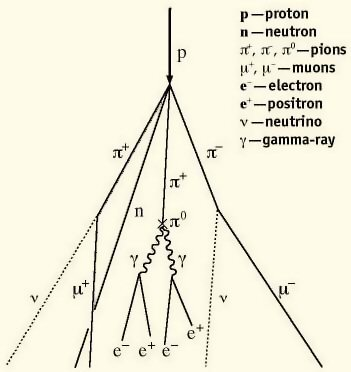
\includegraphics[width=0.5\linewidth]{showers.jpg} 
    \caption{} 
    \label{fg:shower} 
\end{figure}

\section{Resultados de las simulaciones}

En esta sección, se muestran los resultados de las reconstrucciones que hemos estimado para los detectores \textsc{tragaldabas} y \textsc{stratos} . Sus configuraciones respectivas se muestran en las figuras \ref{fg:tragas_rpc} y \ref{fg:stratos_rpc}.

\begin{figure}[H]  % La "H" es para que se queden fijados en este mismo sitio. Para dejar decidir a LaTeX utilizar "ht"
  \begin{subfigure}[b]{0.5\linewidth}
    \centering
    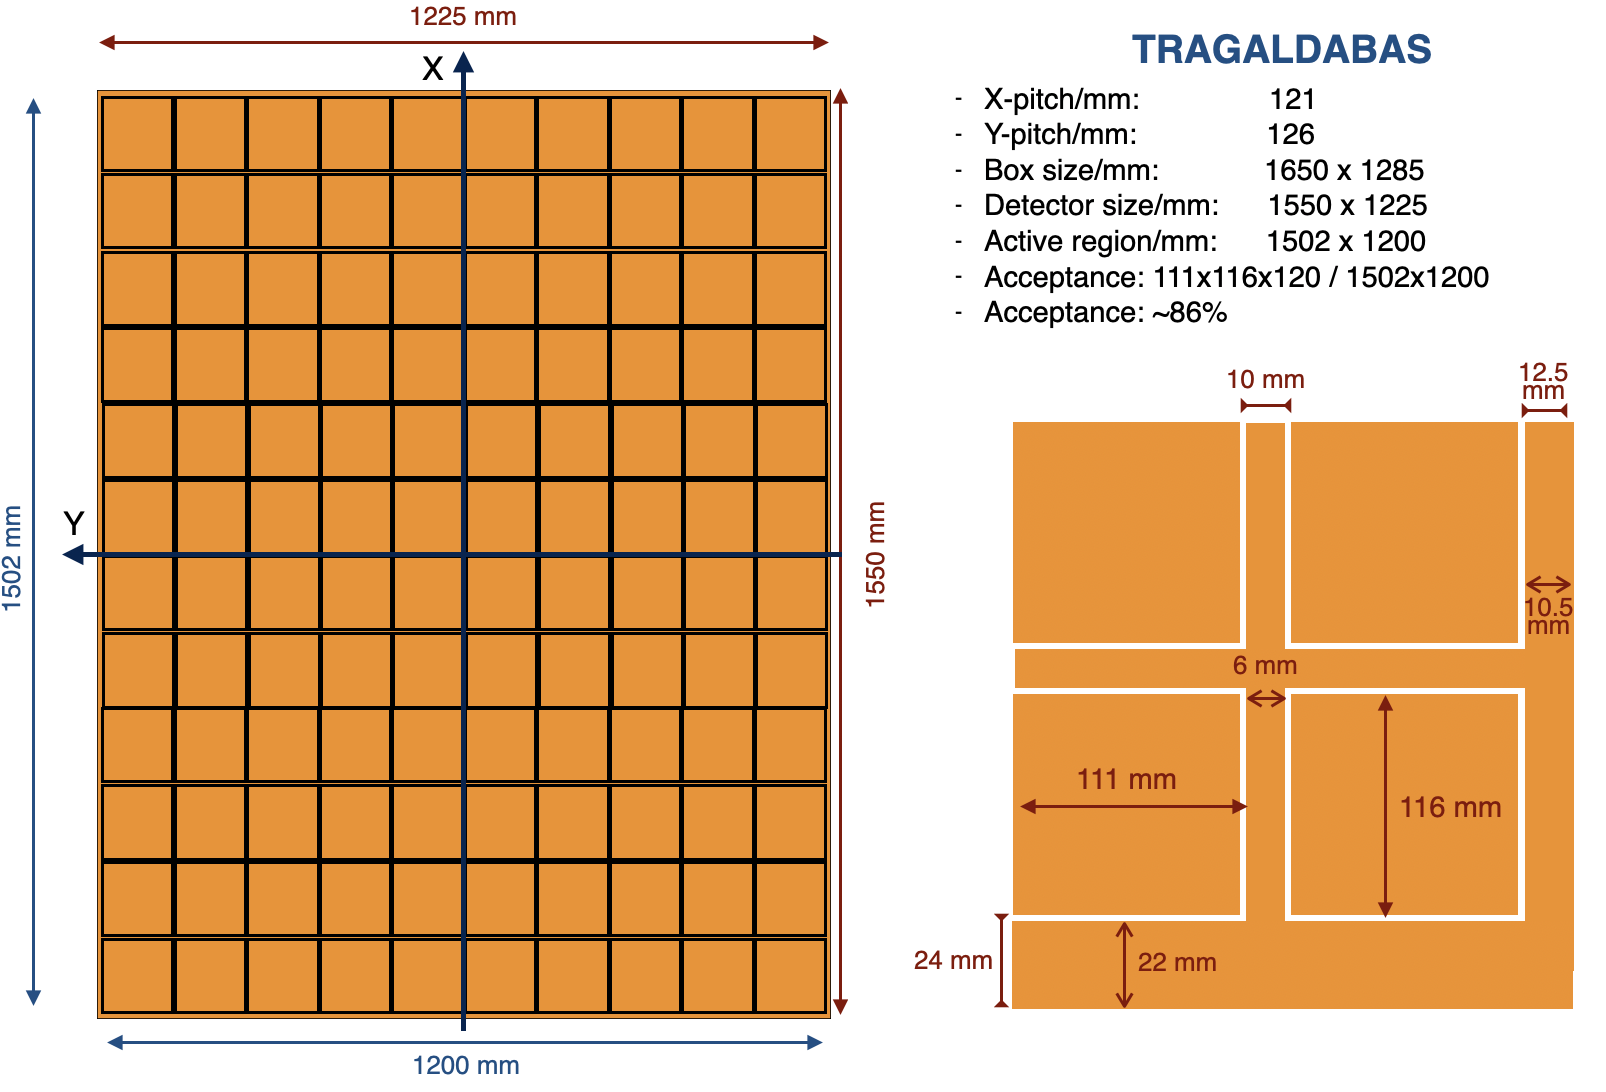
\includegraphics[width=\linewidth]{tragas_pitch.png} 
    \caption{} 
    \label{fg:tragas_rpc} 
  \end{subfigure}%% 
  \begin{subfigure}[b]{0.5\linewidth}
    \centering
    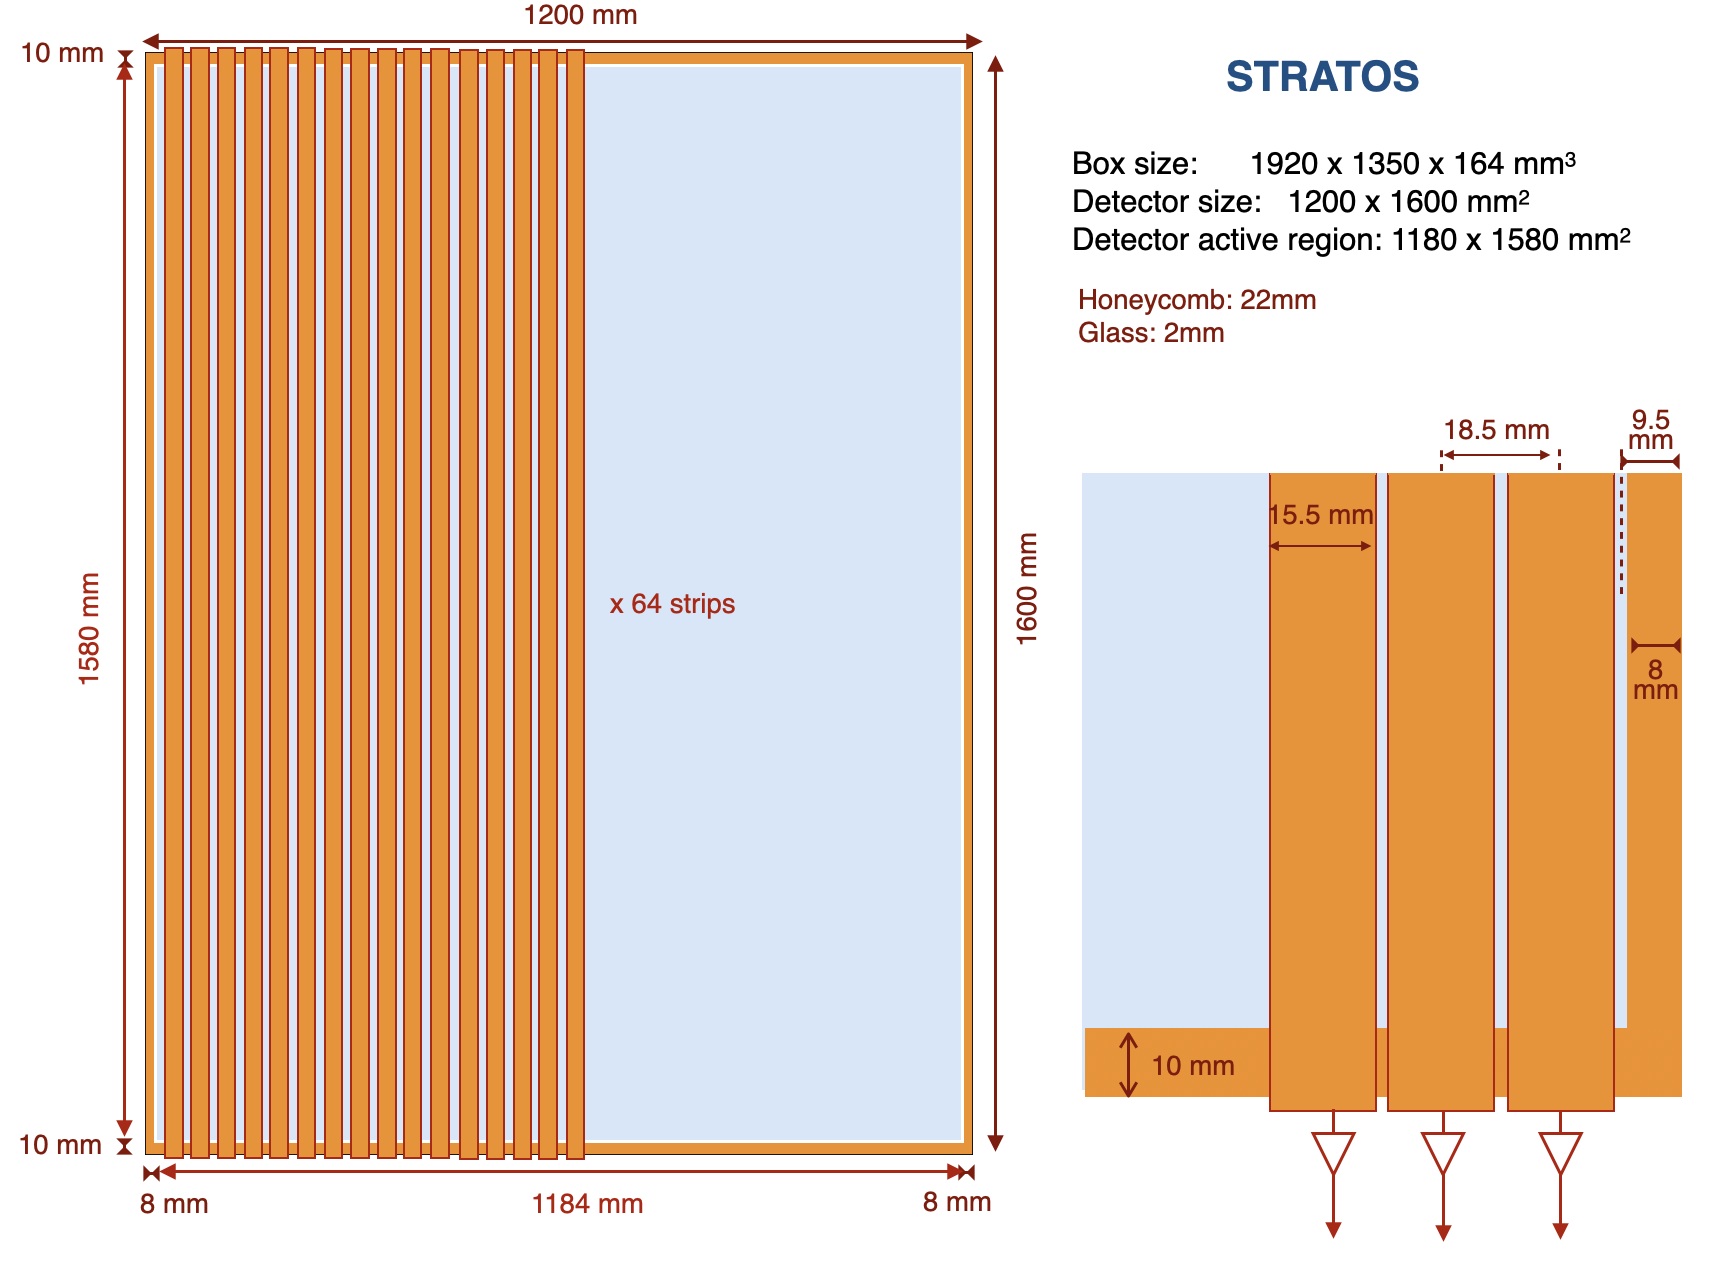
\includegraphics[width=\linewidth]{stratos_pitch.png} 
    \caption{} 
    \label{fg:stratos_rpc} 
  \end{subfigure} 
  \caption{Topología de las RPCs de \textsc{tragaldabas} y \textsc{stratos} respectivamente.}
  \label{fg:tragastratos} 
\end{figure}

Hemos probado su correcto funcionamiento hasta hasta un número máximo de cinco trazas sin que las prestaciones se vean afectadas dada la gran granularidad que tienen ambo detectores. Es de destacar que, de acuerdo con las medidas previas hechas con el detector \textsc{tragaldabas}, la proporción de eventos con mas de 5 partículas simultáneas apenas representarán menos del 1 \% de la muestra total.  Por el contrario, el mayor rato será reconstruir cascadas complejas de partículas en las que los electrones de alta energía puedan dar lugar a cascadas electromagnéticas  como las que se muestran en la figura \ref{fg:shower}. Este es un proceso mas complicado de estudiar de forma automática y forma parte de la lista de prioridades generales del proyecto \textsc{stratos}.


\subsection{Representación gráfica}

Esta versión de genedigitana tiene la opción de mostrar los resultados del proceso en forma de gráfico en 3D, donde las trazas reconstruídas se muestran como líneas continuas, las trazas simuladas como líneas discontínuas, y en color morado se intuye la topología de cada detector. Estas líneas contínuas que representan las trazas reconstruídas, se colorean siguiendo un gradiente desde rojo a amarillo según el valor de $\chi^2$ obtenido en la reconstrucción, siendo el color rojo para la mejor reconstrucción y el amarillo para la peor.


\begin{figure}[H]  % La "H" es para que se queden fijados en este mismo sitio. Para dejar decidir a LaTeX utilizar "ht"
  \begin{subfigure}[b]{0.5\linewidth}
    \centering
    % NOTE:          trim={<left> <lower> <right> <upper>}
    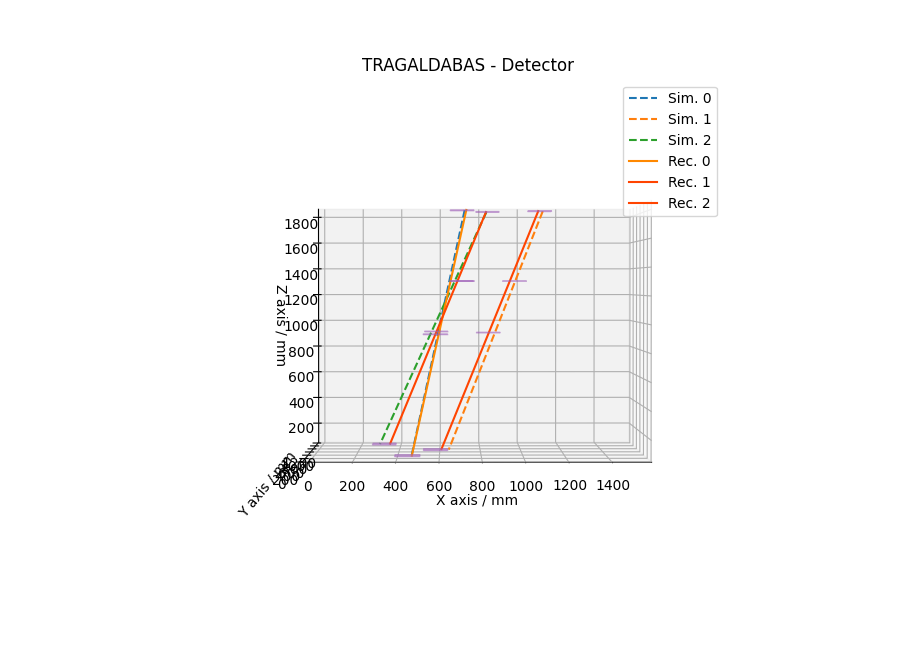
\includegraphics[trim={4cm 3cm 3.9cm 1.9cm},clip,width=\linewidth]  {tragaldabas_xproj.png} 
    \caption{Proyección sobre el eje X.} 
    \label{fg:3-a} 
  \end{subfigure}%% 
  \begin{subfigure}[b]{0.5\linewidth}
    \centering
    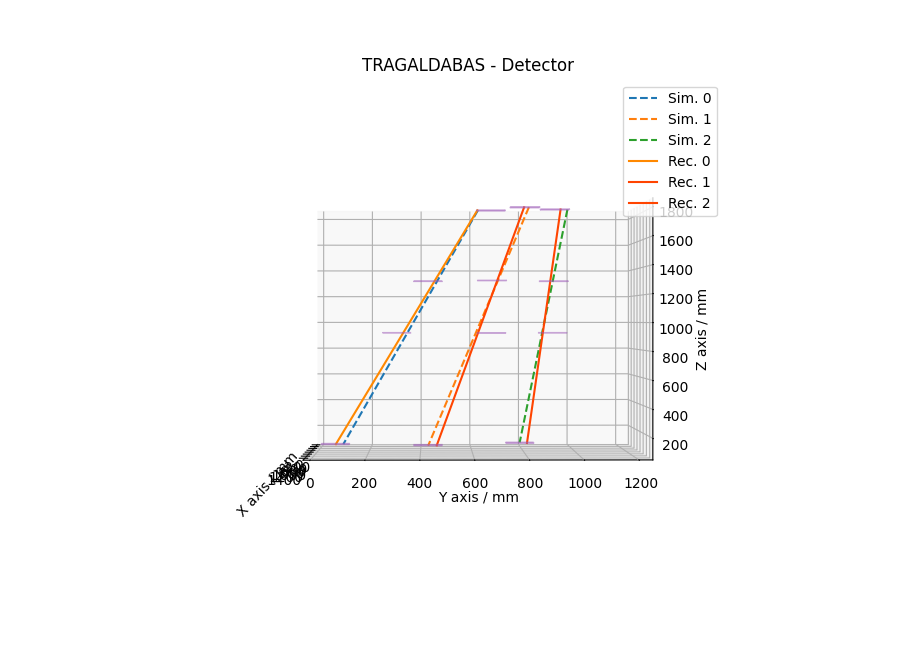
\includegraphics[trim={4cm 3cm 3.9cm 1.9cm},clip,width=\linewidth]  {tragaldabas_yproj.png} 
    \caption{Proyecctión sobre el eje Y.} 
    \label{fg:3-b} 
  \end{subfigure} 
  \begin{subfigure}[b]{0.5\linewidth}
    \centering
    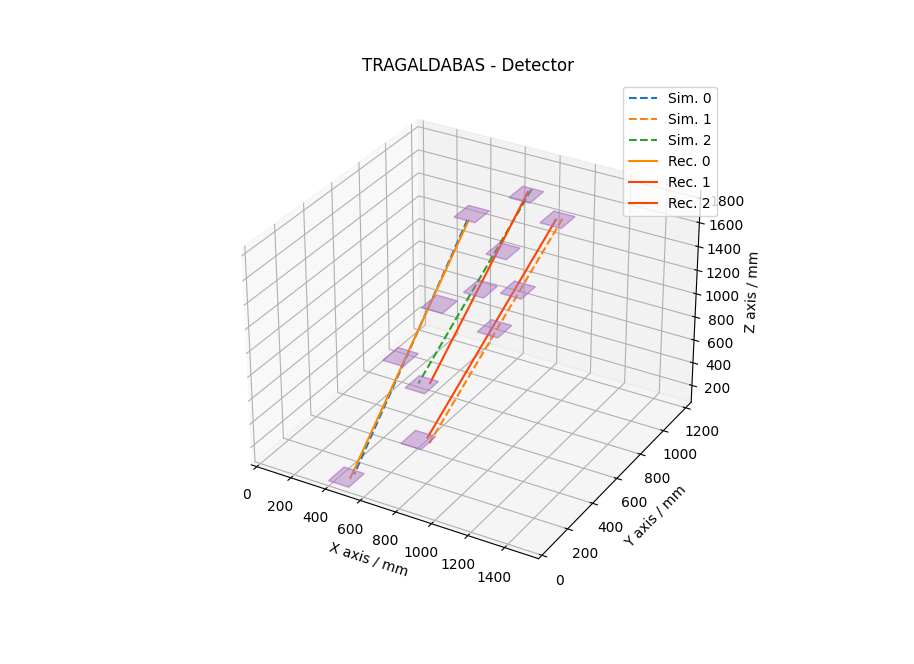
\includegraphics[trim={3.5cm 1cm 2.5cm 1.9cm},clip,width=\linewidth]{tragaldabas_angle1.png} 
    \caption{} 
    \label{fg:3-c} 
  \end{subfigure}%% 
  \begin{subfigure}[b]{0.5\linewidth}
    \centering
    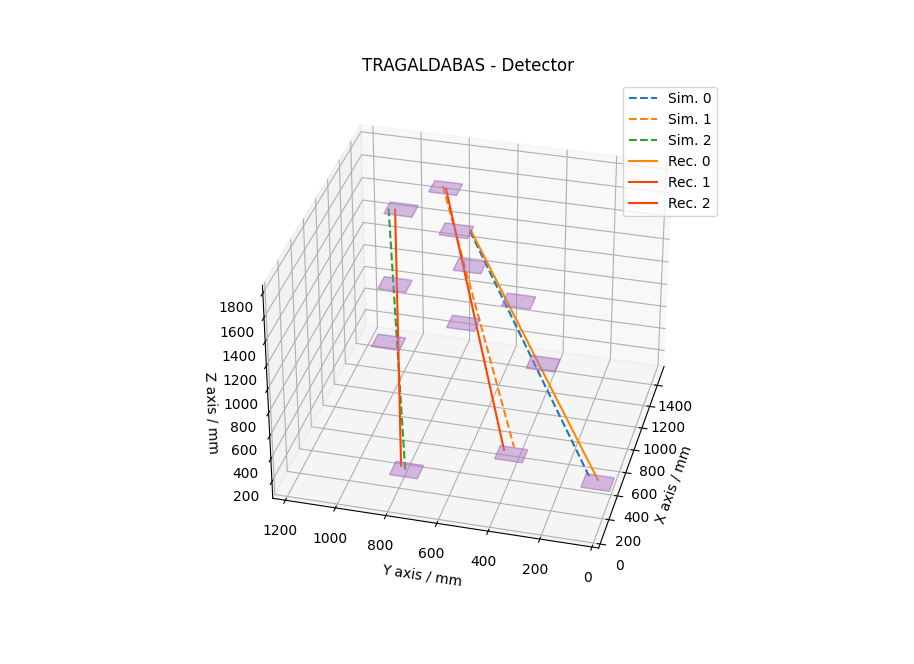
\includegraphics[trim={2.5cm 1cm 2.5cm 1.9cm},clip,width=\linewidth]{tragaldabas_angle2.png} 
    \caption{} 
    \label{fg:3-d} 
  \end{subfigure} 
  \caption{Evento de tres trazas en \textsc{tragaldabas} reconstruido.}
  \label{fg:3} 
\end{figure}

En la figura \ref{fg:3} está representado un evento en \textsc{tragaldabas} con tres trazas que se reconstruyen sin dificultad. Se puede ver en las proyecciones sobre el plano XZ (figura \ref{fg:3-a}) y el plano YZ (figura \ref{fg:3-b}), así como en perspectiva (figuras \ref{fg:3-c} y \ref{fg:3-d}). 


\begin{figure}[H] 
  \begin{subfigure}[b]{0.5\linewidth}
    \centering
    % NOTE:          trim={<left> <lower> <right> <upper>}
    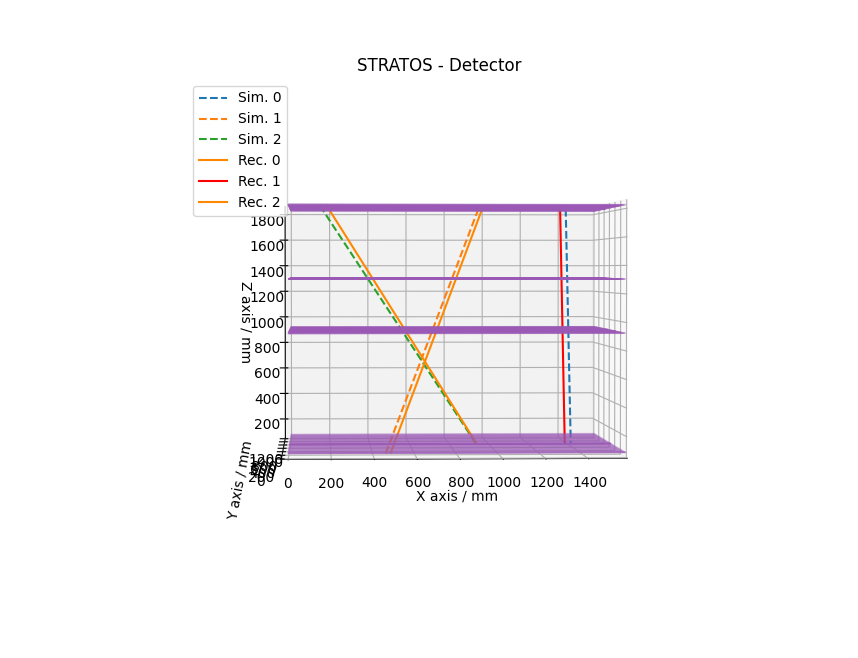
\includegraphics[trim={4cm 3cm 3.9cm 1.9cm},clip,width=\linewidth]  {stratos_xproj.png} 
    \caption{Proyecctión sobre el eje X.} 
    \label{fg:4-a} 
  \end{subfigure}%% 
  \begin{subfigure}[b]{0.5\linewidth}
    \centering
    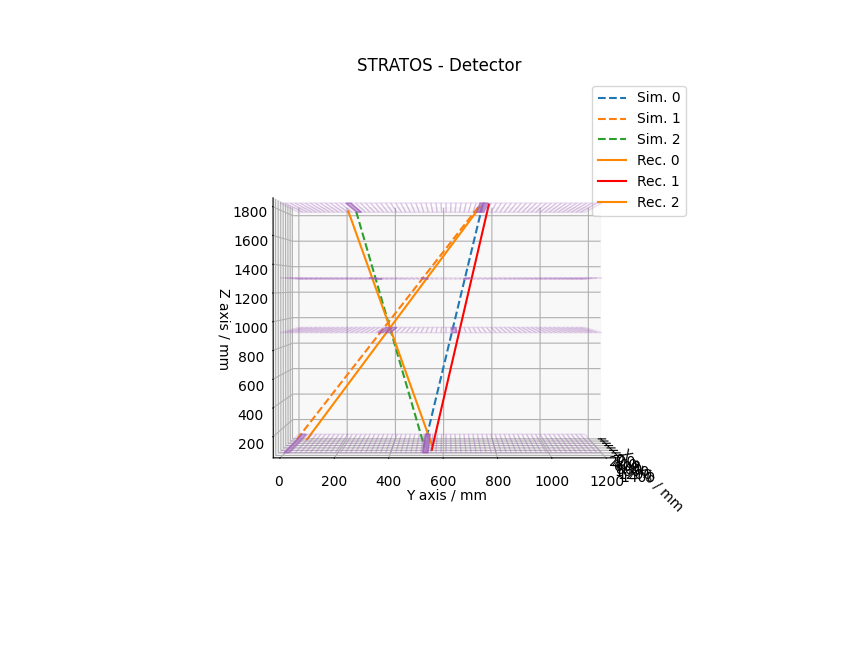
\includegraphics[trim={4cm 3cm 3.9cm 1.9cm},clip,width=\linewidth]  {stratos_yproj.png} 
    \caption{Proyecctión sobre el eje Y.} 
    \label{fg:4-b} 
  \end{subfigure} 
  \begin{subfigure}[b]{0.5\linewidth}
    \centering
    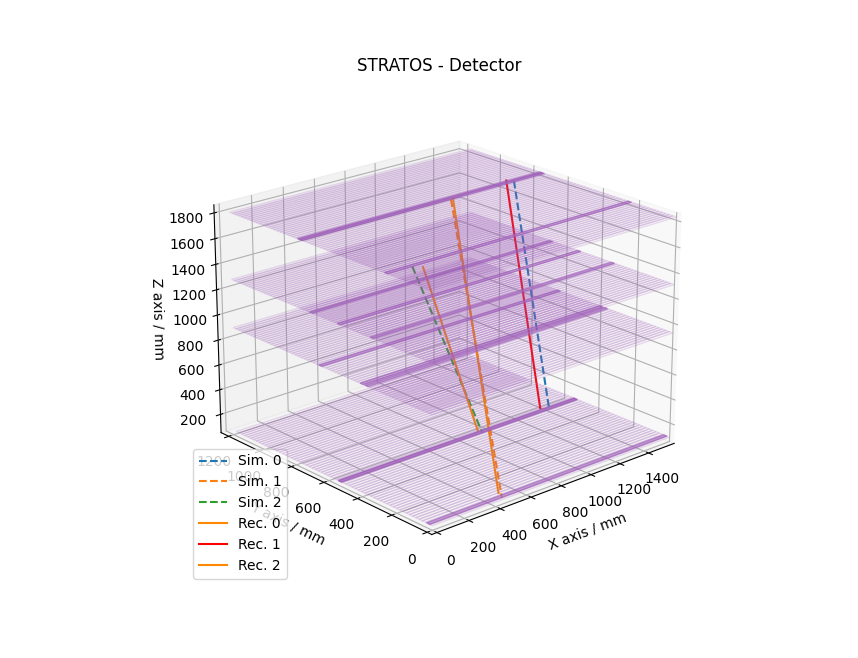
\includegraphics[trim={3.5cm 1cm 2.5cm 1.9cm},clip,width=\linewidth]{stratos_angle1.png} 
    \caption{} 
    \label{fg:4-c} 
  \end{subfigure}%% 
  \begin{subfigure}[b]{0.5\linewidth}
    \centering
    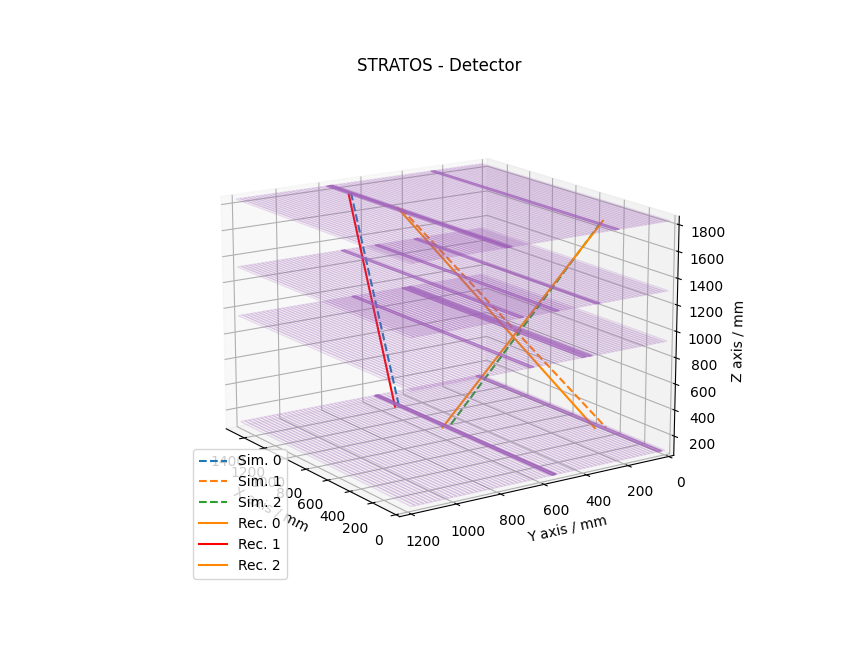
\includegraphics[trim={2.5cm 1cm 2.5cm 1.9cm},clip,width=\linewidth]{stratos_angle2.png} 
    \caption{} 
    \label{fg:4-d} 
  \end{subfigure} 
  \caption{Evento de tres trazas en \textsc{stratos} reconstruido.}
  \label{fg:4} 
\end{figure}

Como se puede observar en la figura \ref{fg:4} que representa otro evento diferente simulado para el detector \textsc{stratos}, las imágenes están colocadas de la misma forma.

El detector \textsc{stratos} tiene 64 conductores en cada plano colocados de forma paralela entre sí que legan de un extremo a otro llamados \textit{strips}. La posición del hit en el eje Y se determina por el \textit{strip} que recibe la señal. La posición en el eje X en cambio, se determina por el tiempo que dicha señal tarda en recorrer todo el conductor. El proceso de simulación para este detector es el mismo que para \textsc{tragaldabas}, así como la reconstrucción una vez obtenidas las posiciones $(x, y)$ en cada plano digitalizadas.

\subsection{Resultados numéricos}

Finalmente, se muestra a continuación como ejemplo algunos de los datos generados y reconstruídos para ambos detectores.

\begin{figure}[H] 
  \centering
  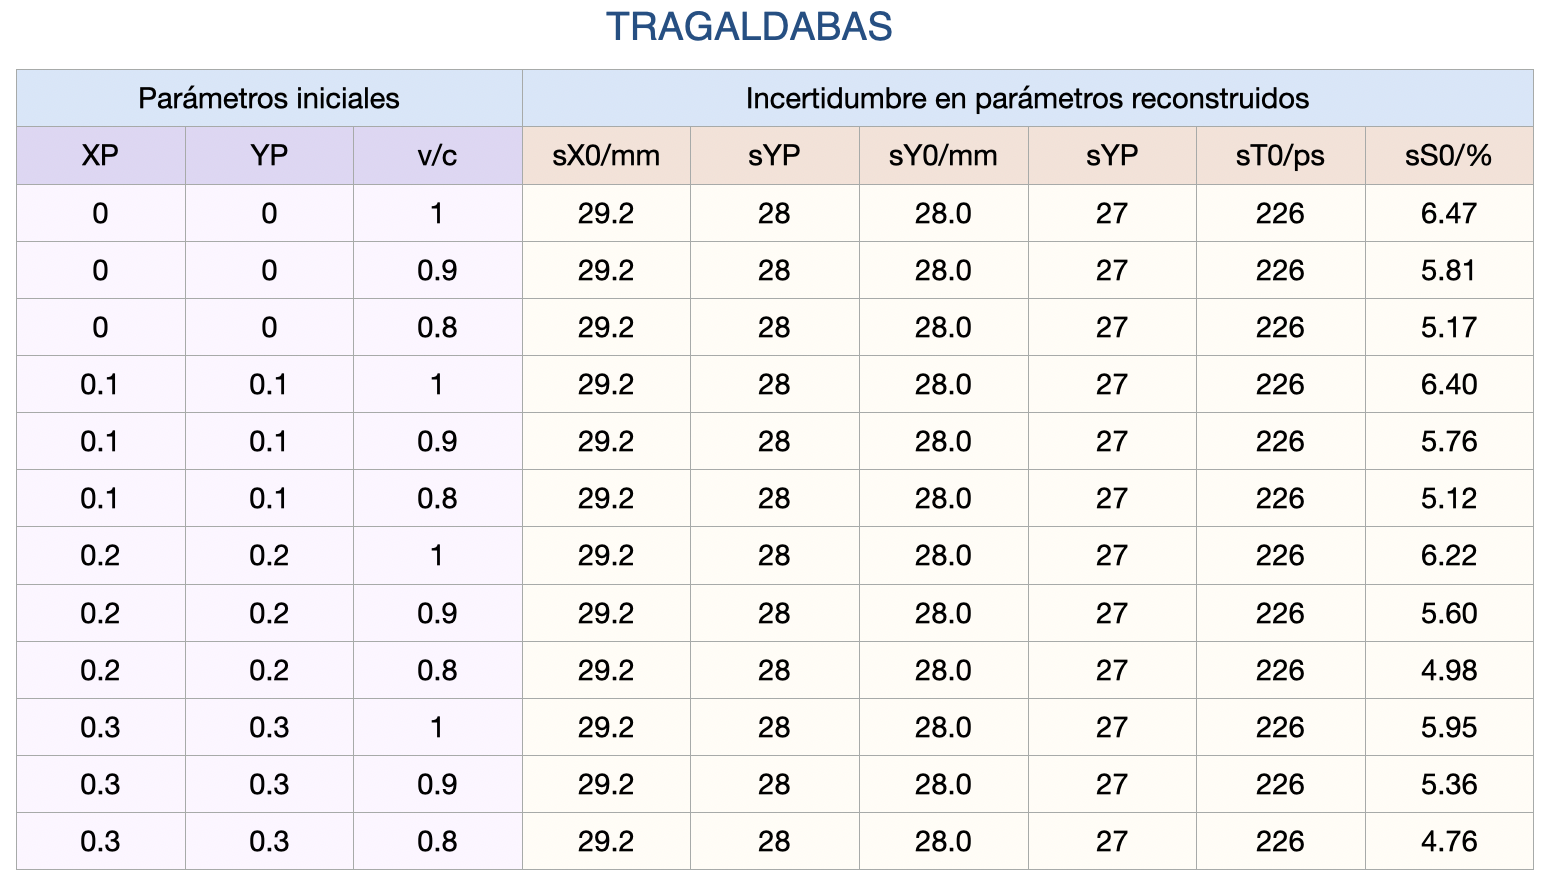
\includegraphics[width=\linewidth]{tabla_param_tragas.png} 
  \caption{Datos de la reconstrucción en el detector \textsc{tragaldabas}.}
  \label{fg:datos_tragas} 
\end{figure}


\begin{figure}[H] 
  \centering
  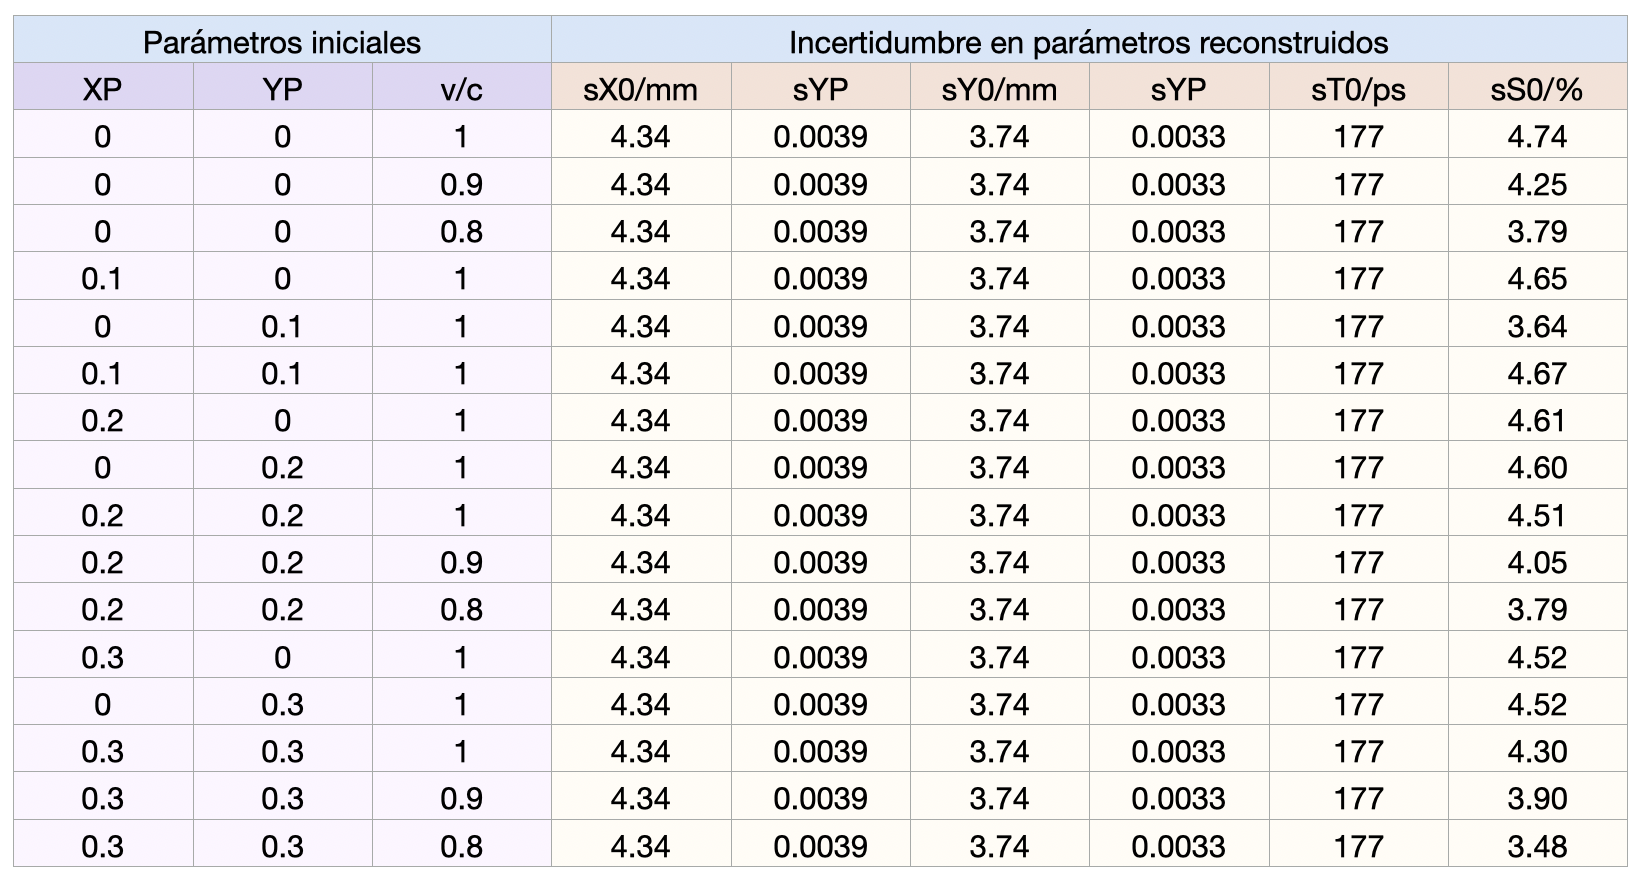
\includegraphics[width=\linewidth]{tabla_param_stratos.png} 
  \caption{Datos de la reconstrucción en el detector \textsc{stratos}.}
  \label{fg:datos_stratos} 
\end{figure}

\section{Apéndice}

\subsection{Código para la reconstrucción}

El código destinado a la reconstrucción para este estudio se puede encontrar en el repositorio público de GitHub:

\url{https://github.com/MCruces-fz/TRAGALDABAS-Kalman-Filter/tree/first_reconstruction}

Aquí se pueden leer las clases utilizadas y mencionadas en este documento, así como interpretar el software con \textsf{Python 3}.


\begin{thebibliography}{9}
    \bibitem{yafonbar}
    \textbf{Studies on the Composition and Energy of Secondary Cosmic Rays with the Tragaldabas Detector}\\
    \textit{Yanis Fontela Barba}, departamento de Física de Partículas.\\
    \textsf{Universidade de Santiago de Compostela}

    \bibitem{joaneh}
    \textbf{The Kalman Filter Technique applied to Track Fitting in GLAST}\\
    \textit{Jose A. Hernando}, Santa Cruz Institute for Particle Physics.\\
    \textsf{University of California. Santa Cruz}

    \bibitem{jag}
    \textbf{jag}\\
    \textit{Jose A. Garzón}, ....\\
    \textsf{...}

    \bibitem{moscu}
    \textbf{Moscú}\\
    \textit{Jose A. Garzón}, ....\\
    \textsf{...}

    \bibitem{ttrack}
    \textbf{Tim Track}\\
    \textit{Jose A. Garzón}, ....\\
    \textsf{...}
\end{thebibliography}



\end{document}

% Basurilla


para una altura concreta definida por el índice $k$ y siendo $v_k$ la velocidad de la partícula. El cuadro \ref{tb:planos} muestra estos datos de los planos.

\begin{table}
\centering
\begin{tabular}{@{}crrc@{}}
\toprule
Nombre & Altura   & $z$   & $k$   \\ \midrule
T1     & 1826     & 0     & 3     \\
T2     & 1304     & 522   & 2     \\
T3     & 924      & 902   & 1     \\
T4     & 87       & 1739  & 0     \\ \bottomrule
\end{tabular}
\caption{Los cuatro planos de \textsc{tragaldabas}, con alturas y coordenadas $z$ en mm.}
\label{tb:planos}
\end{table}



